\begin{figure*}
\begin{subfigure}[t]{0.32\textwidth}
    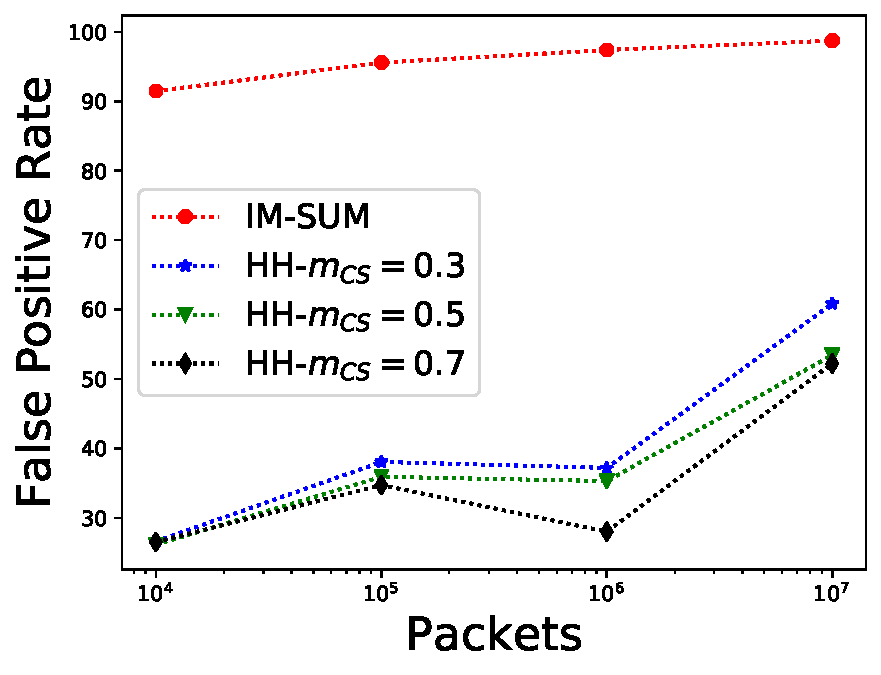
\includegraphics[width=\linewidth]{HH/figures/FPR_per_pkts_m=0.03125.pdf}
    \caption{32KB}
    \label{fig:fig3_a}    
\end{subfigure}\hfill
\begin{subfigure}[t]{0.32\textwidth}
    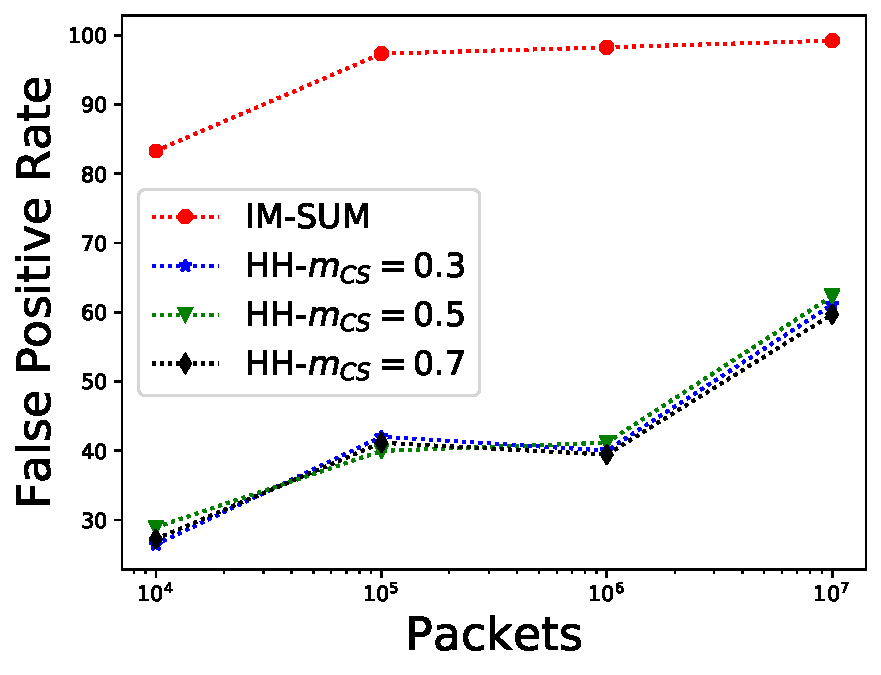
\includegraphics[width=\linewidth]{HH/figures/FPR_per_pkts_m=0.0625.pdf}
    \caption{64KB}
    \label{fig:fig3_b}
\end{subfigure}\hfill
\begin{subfigure}[t]{0.32\textwidth}
    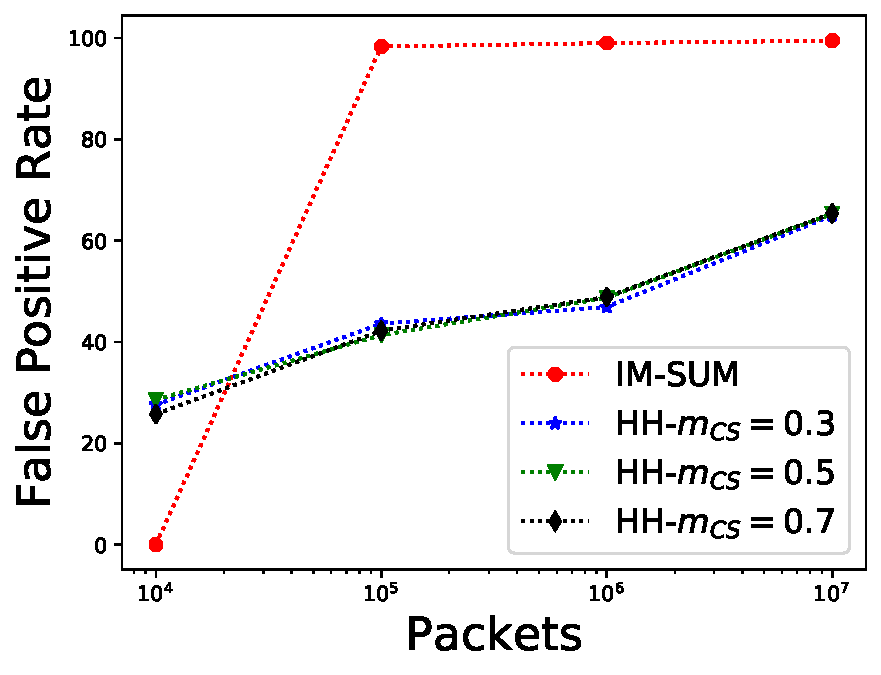
\includegraphics[width=\linewidth]{HH/figures/FPR_per_pkts_m=0.125.pdf}
    \caption{128KB}
    \label{fig:fig3_c}
\end{subfigure}

\begin{subfigure}[t]{0.32\textwidth}
    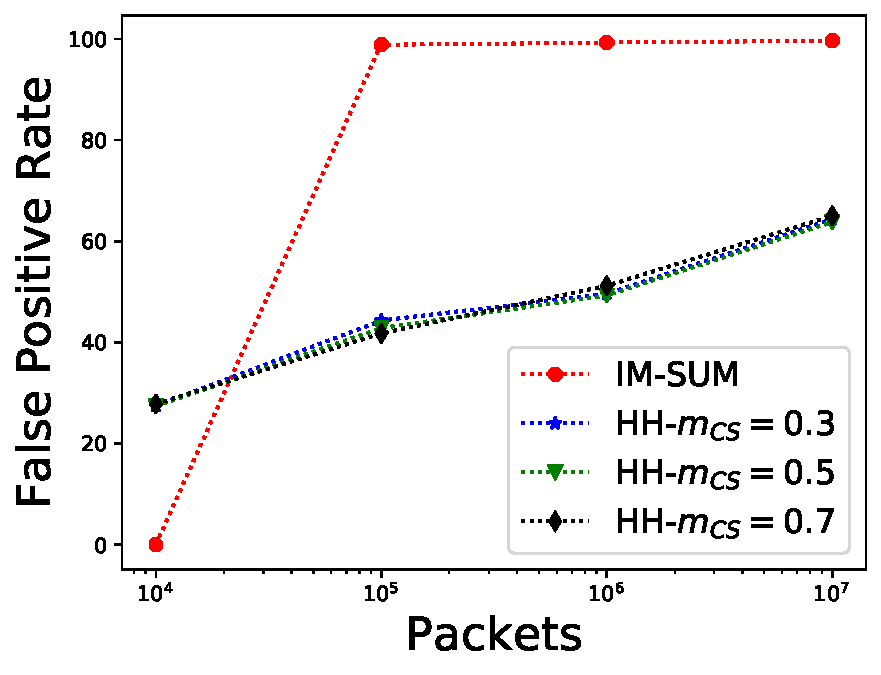
\includegraphics[width=\linewidth]{HH/figures/FPR_per_pkts_m=0.25.pdf}
    \caption{0.25MB}
    \label{fig:fig3_d}
\end{subfigure}\hfill
\begin{subfigure}[t]{0.32\textwidth}
    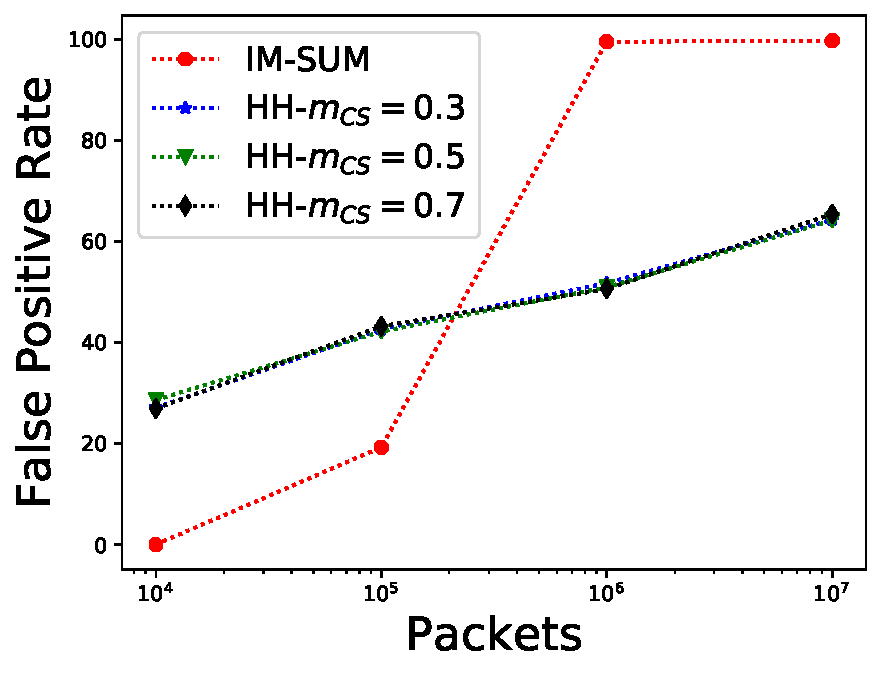
\includegraphics[width=\linewidth]{HH/figures/FPR_per_pkts_m=0.5.pdf}
    \caption{0.5MB}
    \label{fig:fig3_e}
\end{subfigure}\hfill
\begin{subfigure}[t]{0.32\textwidth}
    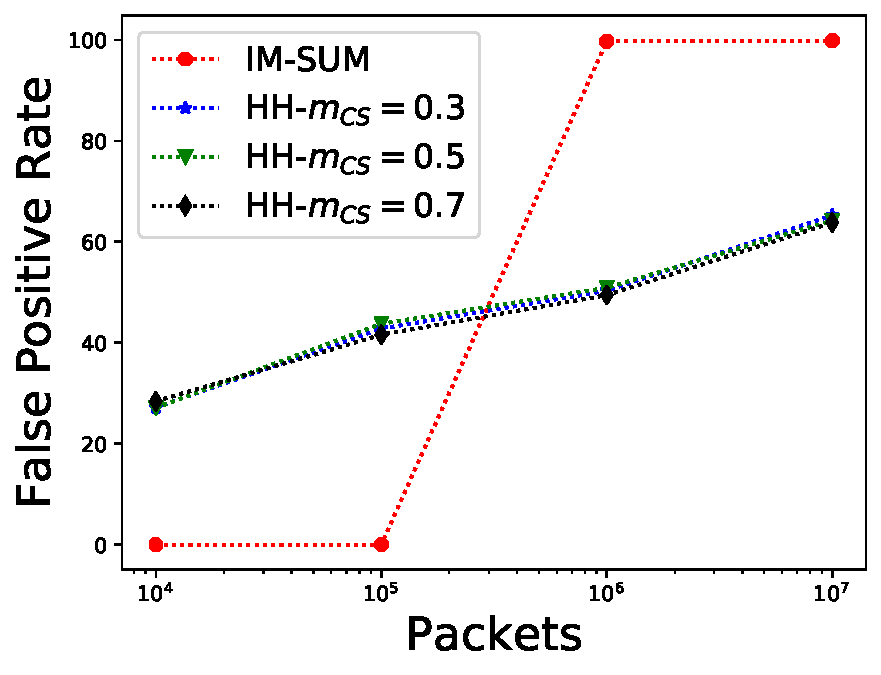
\includegraphics[width=\linewidth]{HH/figures/FPR_per_pkts_m=1.0.pdf}
    \caption{1MB}
    \label{fig:fig3_f}
\end{subfigure}

\caption{The Average False Positive Rate as function of number of packets, comparing our algorithm in three different settings vs. the Elephants algorithm for $\phi=0.001,\delta=0.05$}
\label{figure3}
\end{figure*}